\chapter{M\'odulos}
\label{chap:modulos}

En \'este cap\'itulo se dar\'a una descripci\'on general de los m\'odulos con los que cuenta lpmd, as\'i como tambi\'en propiedades de los mismos, no todos tendr\'an ejemplos, m\'as bien se pretende dar una descripci\'on de lo que es capaz de realizar cada m\'odulo, sin embargo puede encontrar muchos ejemplos en el cap\'itulo~\ref{chap:exa}.

A continuaci\'on veremos los m\'odulos y sus detalles dependiendo de su tipo, en cada una de las secciones siguientes.

%%%%%%%%%%%%%%%%%%%%%%%%%%%%%%%%%%%%%%%%%%%%%%%%%%%%%%%%%%%%%%%%%
%%%%%%%%%%%%%%%%%%%%%%%%%%%%%%%%%%%%%%%%%%%%%%%%%%%%%%%%%%%%%%%%%
\section{M\'odulos Entrada/Salida}
\label{chap:modulos:entradasalida}
Estos m\'odulos pueden ser cargados por \verb|input| y \verb|output|, por lo que los argumentos necesitan ser entregados en esta misma linea. Es decir la instrucci\'on ser\'a siempre de la forma:

\control{input module=mod file=.. opc1=.. ...  opcN=...}
\control{output module=mod file=.. opc1=.. ... opcN=...}

en donde \verb|opcX| son las opciones de cada m\'odulo en paticular, siendo \verb|file| una opci\'on com\'un a la mayot\'ia de los m\'opdulos de entrada/salida.

\subsection{dlpoly}
Este plugin, pretende dar una soluci\'on tipica y eficiente a los archivos de entrada que el usuario ya posee en \verb|dlpoly| y que el trabajo de migrar estos archivos a otras configuraciones podria implicar una inversion de tiempo.

Con el m\'odulo \verb|dlpoly|, se pueden cambiar los archivos de configuracion cristalina de \verb|dlpoly| (\verb|HISTORY| o \verb|CONFIG|) a cualquier otro m\'odulo y viceversa. Los argumentos utilizados por el m\'odulo \verb|dlpoly| son:

\fb{
\begin{tabular}{lcl}
 file & = & Archivo que contiene la configuraci\'on \\
 &&de \textbf{dlpoly}\\
 level & = & Nivel del archivo (0,1,2).\\
 preiodicity & = & Especifica \textit{key} de periodicidad del \\
 &&fichero CONFIG.\\
 ftype & = & Especif\'ica el typo de archivo, \texttt{HISTORY} o\\
 &&\texttt{CONFIG}, a ser le\'ido.\\
\end{tabular}
}

\subsection{lpmd}\label{subsec:lpmdformato}

Es un formato propio de {\lpmd}, tiene la ventaja de que no s\'olo guarda la informaci\'on de las posiciones at\'omicas de las part\'iculas, sino que adem\'as guarda informaci\'on sobre la celda de simulaci\'on. Las posiciones, a diferencia de \verb|xyz|, se encuentran escaladas, por lo que cuenta con opciones muy simples de manejo, encarecidamente recomendamos su uso para trabajos serios. Adem\'as a partir de la version 0.6.1 de {\lpmd}, este plugin cuenta con la opcion de trabajar directamente formatos comrpimidos con zlib. Entre las opciones principales destacan

\fb{
\begin{tabular}{lcl}
 file & = & archivo de entrada/salida.\\
 level & = & indica el nivel del fichero, estos pueden ser \\
           &&0(pos),1(pos y vel) y 2(pos,vel y ace).\\
 extra & = & Informaci\'on extra en el fichero sobre los \'atomos \\
           &&rgb, type, etc.\\
 type & = & Especif\'ica el tipo de fichero, \texttt{lpmd}(default) o \\
           &&\texttt{zlp}.\\
 blocksize & = & tamaño del \textit{block} de compresi\'on cuando es \\
           &&del tipo \texttt{zlp}.\\ 
\end{tabular}
}

La forma com\'un de uso en lpmd es,

\begin{itemize}
 \item \textbf{Cargando un fichero lpmd}
       \control{input module=lpmd file=archivo.lpmd}
 \item \textbf{Escribiendo la salida en un fichero lpmd con velocidades}
       \control{output module=lpmd file=salida.lpmd level=1}
\end{itemize}

\subsection{vasp}
El plugin, es utilizado para leer ficheros POSCAR de \verb|vasp| como un fichero de configuracion inicial, o bien para otro prop\'osito, entre las opciones del m\'odulo, estan:

\fb{
\begin{tabular}{lcl}
 file & = & Archivo que contiene la configuracion de \textbf{dlpoly}\\
 species & = & lista de las especies (en orden) del fichero \\
 &&POSCAR.\\
 level & = & Especif\'ica el nivel del archivo.\\
 type & = & Tipo de posiciones, direct/cartesian.\\
\end{tabular}
}

\subsection{xyz}
\'Este es el m\'odulo que se utiliza para cargar/escribir archivos de configuraci\'on en formato \verb|xyz|, las opciones actuales de este m\'odulo son :

\fb{
\begin{tabular}{lcl}
 file & = & archivo de entrada/salida.\\
 level & = & indica el nivel del fichero, estos pueden ser \\
           &&0(pos),1(pos y vel) y 2(pos,vel y ace).\\
 coords & = & utilizado para ``posicionar'' una celda que \\
           &&ha sido leida, sus valores pueden ser \\
           &&centered/uncentered.\\
 inside & = & Puede ser true/false, indica si los \'atomos que \\
          &&est\'an fuera de una celda se deben reubicar.\\
 external & = & ignore/consider. Espec\'ifica si se deben ignorar \\
          &&o considerar los atomos fuera de la celda.\\
\end{tabular}
}

Muchas de estas opciones no son utilizadas en una corrida con {\lpmd}, sin embargo pueden ser utiles a la hora de trabajar con utilidades tales como \verb|lpmd-analyzer| u otras. En general la forma de utilizar el m\'odulo es,

\begin{itemize}
 \item \textbf{Cargando un fichero xyz}
       \control{input module=xyz file=archivo.xyz}
 \item \textbf{Escribiendo la salida en un fichero xyz con velocidades}
       \control{output module=xyz file=salida.xyz level=1}
\end{itemize}

No todas las opciones son necesarias, muchas de ellas ya tienen valores por defecto, vease \verb|lpmd -p xyz| para m\'as informaci\'on.

\subsection{mol2}
Utilizado para lectura/escritura de fichefros de tipo \verb|mol2|, el soporte, al igual que el formato \verb|pdb| es b\'asico sin embargo es \'util para convertir nuestras configuraciones.

entre las opciones t\'ipicas de \verb|mol2| encontramos :

\fb{
\begin{tabular}{lcl}
 file & = & Archivo que contiene la configuracion at\'omica\\
\end{tabular}
}

\subsection{pdb}
Utilizado para lectura/escritura de archivos de tipo \verb|pdb|, el soporte actual de este tipos de ficheros es b\'asico, sin embargo puede ser \'util para convertir ficheros para la visualizaci\'on con otros programas.

Entre las opciones t\'ipicas de \verb|pdb| est\'an :

\fb{
\begin{tabular}{lcl}
 file & = & Archivo que contiene la configuracion at\'omica\\
\end{tabular}
}

\subsection{rawbinary}
Utilizado para lectura/escritura de archivos de tipo binario, son eficientes para grandes set de configuraciones, es similar al antiguo formato \verb|lpmd 1.0| pero escrito de forma binaria, lo que agiliza cualquier an\'alisis que se desee llevar a cabo.

Entre las opciones t\'ipicas de \verb|rawbinary| est\'an :

\fb{
\begin{tabular}{lcl}
 file & = & Archivo que contiene la configuracion at\'omica\\
 level & = & Especif\'ica el nivel del archivo.\\
\end{tabular}
}

Generalmente este archivo es utilizado para analisis sobre configuraciones muy grandes, para reducir el tiempo de an\'alisis.

%%%%%%%%%%%%%%%%%%%%%%%%%%%%%%%%%%%%%%%%%%%%%%%%%%%%%%%%%%%%%%%%%
%%%%%%%%%%%%%%%%%%%%%%%%%%%%%%%%%%%%%%%%%%%%%%%%%%%%%%%%%%%%%%%%%
\section{M\'odulos Generadores de Celda}
\label{chap:modulos:generadores}
Estos m\'odulos pueden ser cargados por \verb|input|, por lo que los argumentos necesitan ser entregados en esta misma linea. Es decir la instrucci\'on ser\'a siempre de la forma:

\control{input module=mod opc1=.. ...  opcN=...}

en donde \verb|opcX| son las opciones de cada m\'odulo en paticular. Estos m\'odulos s\'olo \textit{generan} celdas de simulaci\'on, su intenci\'on es hacer celdas de distintos tipos de manera f\'acil y amigable para el usuario. A continuaci\'on listamos los principales generadores de celda.

\subsection{crystal3d}
Genera una celda cristalina tridimiensional. Este m\'odulo se utiliza en lugar de un fichero de entrada, para entregar las posiciones at\'omicas de la red cristalina, 

\fb{
\begin{tabular}{lcl}
 symbol & = & S\'imbolo at\'omico de la especie.\\
 n$\alpha$ & = & $\alpha=x,y,z$ El n\'umero de replicas de la celda base.\\
 type & = & Tipo de celda, fcc, bcc, hcp, etc.\\
\end{tabular}
}

Consideremos por ejemplo una celda c\'ubica de \textbf{Fe} con un tama\~no de 10 \AA por cada lado.

\begin{itemize}
 \item \textbf{Especificamos el detalle del cristal}
       \control{cell crystall a=10 b=10 c=10 alpha=90 beta=90 gamma=90}
 \item \textbf{Generamos una celda  fcc dentro del cristal}
       \control{input module=crystal3d type=fcc symbol=Fe nx=3 ny=3 nz=3}
\end{itemize}

Esto generar\'a entonces una celda cristalina \verb|fcc| con par\'ametro de red $10/3 = 3.33$, para comenzar la simulaci\'on.

\subsection{crystal2d}
A diferencia de los generadores de cristalprevios, este m\'odulo genera cristales simples bidimensionales, los argumentos requeridos para generar son:

\fb{
\begin{tabular}{lcl}
 symbol & = & S\'imbolo at\'omico de la especie.\\
 a & = & Longitud del vector base $\vec{a}$.\\
 b & = & Longitud del vector base $\vec{b}$.\\
 gamma & = & \'Angulo entre los vectores base.\\
 n$\alpha$ & = & $\alpha=x,y$ El inverso sobre el largo del cristal.\\
\end{tabular}
}

Consideremos por ejemplo una celda triangular con atomos de Ar, donde el tamano del cristal es de 10 \AA.

\begin{itemize}
 \item \textbf{Especificamos el detalle del cristal}
       \control{cell crystall a=10 b=10 c=0 alpha=90 beta=90 gamma=90}
 \item \textbf{Generamos una estructura bidimensional dentro del cristal}
       \control{input module=crystal2d a=2 b=2 symbol=Fe gamma=60 nx=2 ny=2}
\end{itemize}

\subsection{voronoi}
Utiliza la construcci\'on de \textbf{voronoi} para generar nanoestructuras de materiales, entre sus principales caracter\'isticas para la generaci\'on de estas nanoestructuras, est\'an :

\fb{
\begin{tabular}{lcl}
 symbol & = & S\'imbolo at\'omico de la especie.\\
 type & = & Especif\'ica el tipo de grano cristalino, fcc, bcc, etc.\\
 a & = & Constante de red del cristal.\\
 grains & = & Cantidad de granos generados dentro de la celda.\\
\end{tabular}
}

Al igual que los m\'etodos generadores de celda previos, el detalle general del cristal es entregado con la orden \verb|cell|, y el resto es especificado por el m\'odulo, consideremos un ejemplo que para hacerlo m\'as vistoso utilizar\'a el plugin lpvisual y el \textit{quick-mode}

\begin{verbatim}
 lpmd-visualizer -i voronoi:symbol=Fe,type=fcc,a=3.62,grains=6 -u lpvisual -L 50,50,50
\end{verbatim}

\begin{figure}[h!]
 \centering
 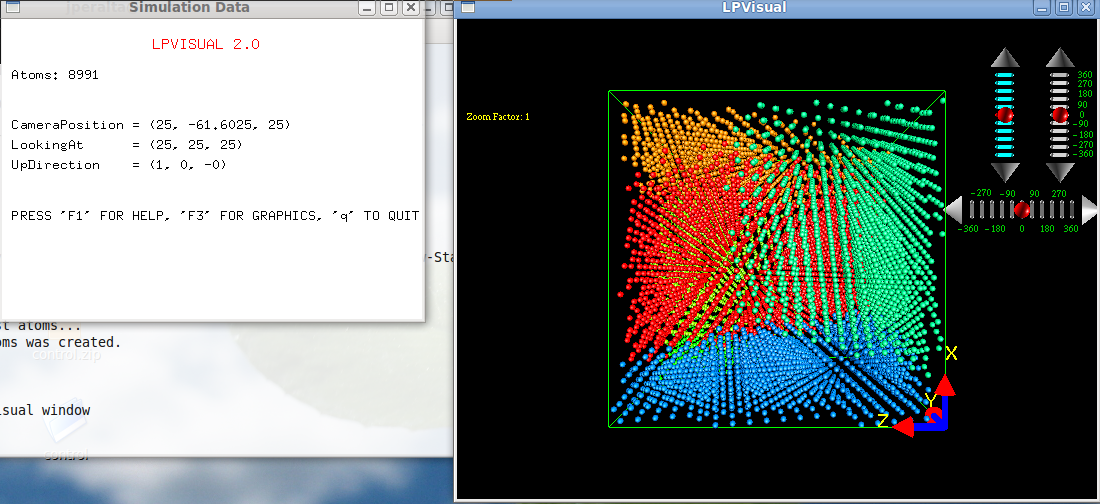
\includegraphics[scale=.35]{voronoi-1.png}
 \label{fig:voronoi-1}
 \caption{Screenshoot de \texttt{lpmd-visusalizer} mostrando una celda generada con voronoi.}
\end{figure}

Podemos ver el resultado de la figura~\ref{fig:voronoi-1}, si esta celda quisieramos guardarla en un formato \verb|lpmd| incluyendo los colores bastar\'ia ejecutarlo con :

 \begin{verbatim}
 lpmd-visualizer -i voronoi:symbol=Fe,type=fcc,a=3.62,grains=6 \
 -u lpvisual -L 50,50,50 -o lpmd:file=new.lpmd,extra=rgb
\end{verbatim}



\subsection{skewstart}
M\'etodo creado por \textit{K. Refson} para el c\'odigo de din\'amica molecular \textbf{moldy}. El objetivo del m\'etodo es generar una configuraci\'on no perdi\'odica suficientemente regulr para garantizar una separaci\'on m\'inima entre los \'atomos. Las opciones junto con la forma de generar una celda con \textit{skewstart}, se describe a continuaci\'on:

\fb{
\begin{tabular}{lcl}
 symbol & = & S\'imbolo at\'omico de la especie.\\
 atoms & = & Especif\'ica el n\'umero de \'atomos dentro \\
 &&de la celda.\\
\end{tabular}
}

Al igual que los m\'etodos generadores de celda previos, el detalle general del cristal es entregado con la orden \verb|cell|, y el resto specificadio por el m\'odulo, consideremos una cleda de arg\'on de 108 \'atomos con un tamano de 20 \AA y que inicializacmos las posiciones at\'omicas con el m\'etodo \textit{skewstart}

\begin{itemize}
 \item \textbf{Especificamos el detalle del cristal}
       \control{cell crystall a=20 b=20 c=20 alpha=90 beta=90 gamma=90}
 \item \textbf{Generamos una celda  fcc dentro del cristal}
       \control{input module=skewstart symbol=Ar}
\end{itemize}
%%%%%%%%%%%%%%%%%%%%%%%%%%%%%%%%%%%%%%%%%%%%%%%%%%%%%%%%%%%%%%%%%
%%%%%%%%%%%%%%%%%%%%%%%%%%%%%%%%%%%%%%%%%%%%%%%%%%%%%%%%%%%%%%%%%
\section{Manejadores de Celda}
Estos m\'odulos son los encargados de generar las \textbf{lista inteligentes} para poder realizar simulaciones o c\'alculos de Din\'amica Molecular, \'estas listas ayudan a reducir el tiempo de c\'alculo utilizado por las simulaciones.

\subsection{linkedcell}
Utiliza el m\'etodo de listas linkeadas, \'este m\'etodo es mucho m\'as rapido que el m\'etodo de m\'inima imagen, y de por s\'i es el m\'as utilizado en la mayor\'ia de los c\'odigos de \textbf{DM}, se puede subdividir la celda a voluntad, sin embargo es recomendable que el tama\~no de subdivisi\'on de la celda no sea menor que la distancia m\'inima de interacci\'on entre las part\'iculas, con algun potencial. Tambi\'en posee el modo \verb|auto| para simplificar la subdivision de la celda.

\begin{itemize}
 \item \textbf{Cargando el M\'odulo}
       \control{use linkedcell \\ cutoff 2.0 \\ nx 10\\ ny 10\\ nz 10\\enduse}
 \item \textbf{Cargando en modo} \texttt{auto}.
       \control{use linkedcell \\ cutoff 2.0 \\ mode auto\\enduse}
 \item \textbf{Aplicando el M\'odulo}
       \control{cellmanager linkedcell}
\end{itemize}

\subsection{minimumimage}
Uiliza el m\'etodo de m\'inima imagen para realizar los procesos. Es mucho m\'as lento que otros m\'etodos, pero en el s\'olo se necesita ingresar el radio de corte del sistema. Este m\'etodo no es bueno cuando el radio de corte es del orden del tama\~no de la mitad de la celda de simulaci\'on.

\begin{itemize}
 \item \textbf{Cargando el M\'odulo}
       \control{use minimumimage \\ cutoff 2.0 \\enduse}
 \item \textbf{Aplicando el M\'odulo}
       \control{cellmanager minimumimage}
\end{itemize}

Con \'esto nuestra simulaci\'on utilizar\'a el m\'etodo de m\'inima imagen para un \verb|cutoff| de 2.0 \AA.

\subsection{lcbinary}
Utiliza el m\'etodo de listas linkeadas, pero a diferencia del anterior, este adapta la subdivisi\'on asignada de manera autom\'atica haciendo que no permanezcan m\'as de un \'atomo por celda, pese a ser un metodo simple y \textit{utilizable}, es recomendable que considere el excesivo consumo de \verb|RAM| que \'este acarrea.

\begin{itemize}
 \item \textbf{Cargando el M\'odulo}
       \control{use lcbinary \\ cutoff 2.0 \\ mode auto\\enduse}
 \item \textbf{Aplicando el M\'odulo}
       \control{cellmanager linkedcell}
\end{itemize}

Si usted no tiene claro que tipo de subdivision debe usar recomenadmos encarecidamente que utilize \verb|linkedcell| en modo \verb|auto|.
%%%%%%%%%%%%%%%%%%%%%%%%%%%%%%%%%%%%%%%%%%%%%%%%%%%%%%%%%%%%%%%%%
%%%%%%%%%%%%%%%%%%%%%%%%%%%%%%%%%%%%%%%%%%%%%%%%%%%%%%%%%%%%%%%%%
\section{Filtros}
Estos m\'odulos son los encargados de modificar de cierta forma la celda de simulaci\'on original, pueden ser utilizados para la generaci\'on de celdas complejas. Su intenci\'on es seleccionar \'atomos bajo cierta caracter\'istica.

Es importante destacar que todos los filtros pueden seleccionar adm\'as de forma inversa, por ejemplo en vez de seleecionar los \'atomos que se encuentran dentro de una regi\'on podemos, utilizando la misma regi\'on, seleccionar los \'atomos que no pertenecen a la regi\'on con el flag :

\control{inverse=true}

dentro de las opciones del filtro. Adem\'as estos filtros pueden ser aplicados con excepciones (\verb|except|) lo que les da una flexibilidad a\'un mayor, ejemplos sobre filtros pueden contrarse en el cap\'itulo~\ref{chap:exa}.

\subsection{box}
Selecciona los \'atomos que se encuentran dentro de una regi\'on rectangular definida por el plugin. Las opciones del plugin son

\fb{
\begin{tabular}{lcl}
 x & = & Rango en la direcci\'on \texttt{x}.\\
 y & = & Rango en la direcci\'on \texttt{y}.\\
 x & = & Rango en la direcci\'on \texttt{z}.\\
\end{tabular}
}

Veamos un filtrado t\'ipico utilizando \verb|box|.

\begin{itemize}
 \item \textbf{Eliminando todo excepto los \'atomos pretenecientes a una regi\'on.}
       \control{filter box x=0-5 y=0-6 z=10-15}
\end{itemize}

Con \'esto podemos seleccionar los \'atomos que se encuentran dentro de la regi\'on del espacio definida para cada uno de los ejes de nuestros vectores base.

\subsection{element}
Selecciona a los \'atomos segun el elemento al que pertenecen. Las opciones del plugin \verb|element| est\'an dadas por,

\fb{
\begin{tabular}{lcl}
 symbol & = & S\'imbolo \'atomico de los \'atomos a eliminar.\\
\end{tabular}
}

Consideremos por ejemplo eliminar los \'atomos de \verb|H| de una muestra original, para ello :

\begin{itemize}
 \item \textbf{Eliminando \'atomos de} \texttt{H}.
       \control{filter species symbol=H}
\end{itemize}

As\'i subdividimos la celda en una grilla de 10x10x10. Para generar las listas de vecinos de cada \'atomo.

\subsection{index}
Selecciona a los \'atomos seg\'un su indice, muy utilizado para igualar configuraciones antiguas en donde el orden de los \'atomos señalaba alguna caracter\'istica. Las opciones del plugin \verb|element| est\'an dadas por,

\fb{
\begin{tabular}{lcl}
 index & = & Lista de \'indices at\'omicos.\\
\end{tabular}
}

Consideremos por ejemplo eliminar los atomos del 1 al 3 o bien del 1 al 50:

\begin{itemize}
 \item \textbf{Eliminando \'atomos del 1 al 3}.
       \control{filter index index=1,2,3}
 \item \textbf{Eliminando \'atomos del 1 al 50}.
       \control{filter index index=1-50}
\end{itemize}

\subsection{sphere}
Selecciona a los \'atomos ubicados dentro de una regi''on esf\'erica, las opciones del plugin son :

\fb{
\begin{tabular}{lcl}
 radius & = & Radio de la esfera en \AA.\\
 center & = & Centro de la esfera, anotado como vector <a,b,c>.\\
\end{tabular}
}

Consideremos por ejemplo seleccionar s\'olo los \'atomos pertenecientes a una regi\'on esf\'erica.

\begin{itemize}
 \item \textbf{Selecci\'on esf\'erica} \texttt{H}.
       \control{filter sphere radius=10 center=<50,50,50>}
\end{itemize}

\subsection{tag}
Selecciona a los \'atomos segun alg\'un \verb|tag| que los caracterize, es decir alguna etiqueta propia de los \'atomos, uno puede aplicarle tag a los \'atomos seg\'un nuestras propias necesidades, sin embargo tambi''en existen \verb|tag| propios de {\lpmd}, tales como \verb|fixedpos|, \verb|fixedvel|, etc. Las opciones del plugin son :

\fb{
\begin{tabular}{lcl}
 name & = & Nombre del tag.\\
 value & = & Booleano true o flase, sobre estado del tag.\\
\end{tabular}
}

Consideremos por ejemplo seleccionar los \'atomos que tienen posicion fija

\begin{itemize}
 \item \textbf{Seleccionando \'atomos de posici\'on fija} \texttt{H}.
       \control{filter tag name=fixedpos value=true}
\end{itemize}

%%%%%%%%%%%%%%%%%%%%%%%%%%%%%%%%%%%%%%%%%%%%%%%%%%%%%%%%%%%%%%%%%
%%%%%%%%%%%%%%%%%%%%%%%%%%%%%%%%%%%%%%%%%%%%%%%%%%%%%%%%%%%%%%%%%
\section{Modificadores}

Los plugins modificadores alteran ciertas caracter\'isticas de un set de \'atomos o de la celda de simulaci\'on completa, es decir las modificaciones pueden aplicarse de forma filtrada, por ejemplo :

\control{apply modify-module start=... end=... each=... over filter-module <filter-options>}

Lo que nos da mayor flexibilidad en el manejo de la simulaci\'on. Sin embargo si queremos modificar la celda en su totalidad, podemos usar simplemente :

\control{apply modify-module start=... end=... each=...}

Casos como el escalamiento de celda, solo pueden aplicar de forma \textit{general} sobre la simulaci\'on.

\subsection{berendsen}
\'Este m\'odulo controla o escala la temperatura, al igual que \textbf{tempscaling}, su diferencia es que el m\'etodo es un escalamiento menos \textbf{brusco}, por lo que en ocaciones se consiguen muy buenos resultados y se logra termalizar de manera m\'as eficiente las muestras. 

La ecuaci\'on que describe el termostato de berendsen es :

$$\frac{dT}{dt} = \frac{T_0 - T}{\tau}$$

Los argumentos requeridos por el m\'odulo son:

\fb{
\begin{tabular}{lcl}
 from & = & Desde que temperatura comenzar a aplicar.\\
 to & = & Temperatura final a la que se desea llegar.\\
 tau & = & Intervalo del termostato.\\
\end{tabular}
}

\subsection{cellscaling}
\'Este m\'odulo es un modificador de la celda, en particular, tiene la propiedad de cambiar el tama\~no de la celda durante la simulaci'on, lo que lo hace una herramienta muy util para ver, por ejemplos, comportamiento de materiales bajo distintas densidades durante una sola simulaci\'on. El m\'odulo tiene las siguientes opciones:

\fb{
\begin{tabular}{lcl}
 percent & = & Especifica el porcentaje en el que se variar\'a \\
 &&el largo de la celda.\\
 axis & = & Indica, el eje (x,y o z) en el que se comprimira \\
 &&la celda (all=hidrost\'atico).\\
 constant & = & true/false indica si la modificacion es constante \\
 &&respecto al valor inicial.\\
\end{tabular}
}

Con \'este m\'odulo entonces pdoemos realizar compresi\'on hidrost\'atica o unidireccional, adem\'as de mantener constante o no el intervalo de escalamiento.

\subsection{displace}
M\'odulo que modifica las posiciones at\'omicas del sistema, a partir de un desplazamiento vectorial de los \'atomos de la muestra. Las caractr\'isticas del m\'odulo son :

\fb{
\begin{tabular}{lcl}
 x & = & Desplazamiento en el eje x.\\
 y & = & Desplazamiento en el eje y.\\
 z & = & Desplazamiento en el eje z.\\
\end{tabular}
}

\subsection{moleculecm}
M\'odulo que selecciona moleculas?????? Que hacía este módulo, alguien la puede documentar :).

\subsection{propertycolor}
M\'odulo que asigna colores a los \'atomos segun cierta condici\'on, las opciones principales del plugin son :

\fb{
\begin{tabular}{lcl}
 property & = & Propiedad que se desea colorear.(temperature, velocity, acceleration, neighbours)\\
 min & = & Valor m\'inimo del rango de valores.\\
 max & = & Valor m\'aximo del rango de valores.\\
 cutoff & = & Algunas propiedades necesitan cutoff.\\
 filterby & = & Filtrado por.\\
\end{tabular}
}

Consideremos por ejemplo que deseamos colorear los \'atomos seg\'un su temperatura, y le asociaremos a 300 la temperatura m\'inima y 500 a la m\'axima que ser\'ian los colores del azul al rojo, entonces :

\begin{itemize}
 \item \textbf{Cargamos el modulo}
       \control{use propertycolor as temp\\ min 300\\ max 300\\enduse}
 \item \textbf{Aplicamos coloreado en la simulaci\'on.}
       \control{apply temp start=1 end=1000 each=2}
\end{itemize}

\subsection{quenchedmd}
M\'odulo que m\'inimiza la estructura, utilizando el m\'etodo \textit{Quenched Molecular Dynamics}. Durante el proceso, el integrador no actua como una din\'amica molecular simple, ya que verifica la proyeccion entre fuerza y velocidad, la que se ve forzada si la energ\'ia se incrementa.

\fb{
\begin{tabular}{lcl}
 debug & = & Informaci\'on de debug.\\
\end{tabular}
}

El m\'odulo no necesita argumentos especiales, solo ser llamado y aplicado. Ya que debug es la informaci\'on de depuraci\'on con la que siempre cuentan todos los plugins.

\subsection{randomatom}
M\'odulo que elimina o modifica de forma aleatoria \'atomos de una muestra, sus principales opciones son : 

\fb{
\begin{tabular}{lcl}
 type & = & Tipo de acci\'on delete/replace.\\
 value & = & Valor porcentual de atomos a reemplazar.\\
 symbol & = & S\'imbolo at\'omico, en el caso de reemplazar.\\
 density & = & fixed/free para fijar o no la densidad de la muestra, \'util en modo eliminaci\'on.\\
\end{tabular}
}

Consideremos por ejemplo que deseamos remover \'atomos al azar dentro de un cristal, entonces :

\begin{itemize}
 \item \textbf{Cargamos el m\'odulo}
       \control{use randomatom\\ type delete\\ value 5\\ density fixed\\enduse}
 \item \textbf{Aplicamos coloreado en la simulaci\'on.}
       \control{apply randomatom}
\end{itemize}

la aplicaci\'on tambi\'en puede llevarse acabo en pasos espec\'ificos de la simulaci\'ion, por ejemplo usando \texttt{start=10 end=10 each=1} llevara la eliminaci\'on de \'atomos en ese instante espec\'ifico de la simulaci\'on.

\subsection{replicate}
M\'odulo que replica la celda se simulaci\'on en los distintos ejes, sus opciones principales son

\fb{
\begin{tabular}{lcl}
 nx & = & N\'umero de replicas en la direcci\'on \texttt{x}.\\
 ny & = & N\'umero de replicas en la direcci\'on \texttt{y}.\\
 nz & = & N\'umero de replicas en la direcci\'on \texttt{z}.\\
\end{tabular}
}

Las replicas son n\'umeros enteros de la celda, usualmente este m\'odulo s\'olo se utiliza al comienzo de la simulaci\'on y puede ser llamado con \verb|prepare| para setear previamente la celda. Es importante destacar que la mayor\'ia de las ocaciones que \textbf{utilizan \texttt{prepare replicate}} necesitan desactivar la optimizaci\'on de la celda, por ejemplo :

\begin{itemize}
 \item \textbf{Desactivando optimizaci\'on}
       \control{set optimize-simulation false}
 \item \textbf{Aplicamos replicaci\'on de celda.}
       \control{prepare replicate 2 2 2}
\end{itemize}

Con eso entonces replicamos nuestra celda original dos veces en cada direcci\'on.


\subsection{rotate}
M\'odulo que modifica las posiciones, rotando los \'atomos cierto grado en torno a un origen. Al igual que el m\'odulo \verb|displace|, est\'a desarrollado para la creaci\'on de estructuras m\'as complejas.

\fb{
\begin{tabular}{lcl}
 x & = & Coordenada x del eje de rotaci\'on.\\
 y & = & Coordenada y del eje de rotaci\'on.\\
 z & = & Coordenada z del eje de rotaci\'on.\\
 angle & = & \'Angulo de rotaci\'on en \textbf{grados}.\\
\end{tabular}
}

\subsection{setcolor}
M\'odulo que asigna colores a los \'atomos, es necesario definir colores y con eso aplicarselo a un grupo de \'atomos o bien a todos los \'atomos. 

\fb{
\begin{tabular}{lcl}
 color & = & Vector del color.\\
\end{tabular}
}

Entonces, veamos por ejemplo como asignan un color a todos los \'atomos, recuerde que puede ser aplicado utilizando filtros.

\begin{itemize}
 \item \textbf{Carga el m\'odulo}
       \control{use setcolor as red\\ color <1.0,0.0,0.0>\\enduse}
 \item \textbf{Aplicamos el color}
       \control{apply setcolor}
\end{itemize}

\subsection{settag}
Al igual que la forma de asignar colores a un \'atomo, es posible asignar \verb|tag| o etiquetas a los \'atomos. Entr las opciones del plugin settag estan :

\fb{
\begin{tabular}{lcl}
 name & = & Nombre del tag\\
 value & = & Boleano que indica actividad del tag true/false\\
\end{tabular}
}

De esta forma podemos asignar cualquier tag a los \'atomos. Veamos por ejemplo como asignar \verb|fixedpos| a un set de \'atomos, ser\'ia :

\begin{itemize}
 \item \textbf{Carga el m\'odulo}
       \control{use settag as pos\\ name fixedpos\\ value true\\enduse}
 \item \textbf{Aplicamos el color}
       \control{apply fixedpos}
\end{itemize}

Usualmente las aplicaciones de \verb|settag| o \verb|setcolor| se utilizan fitlrados sobre los \'atomos para llo recuerdo que basta con especificar el filtro dentro de \verb|apply|.

\subsection{setvelocity}
Setea las velocidades de un grupo de \'atomos, los argumentos son :

\fb{
\begin{tabular}{lcl}
 velocity & = & Velocidad a asignar.\\
\end{tabular}
}

Al igual que \verb|setcolor| este plugin puede asignar la velocidad de toda la muestra o de un grupo de \'atomos pertenecientes a ella.

\subsection{shear}
M\'odulo que realiza \textit{shear} (cizalle) sobre la muestra, modificando la forma de la celda, los argumentos principales son :

\fb{
\begin{tabular}{lcl}
 axis & = & Eje en el que se produce el cizalle.\\
 normal & = & Eje perpendicular al eje del cizalle.\\
 strain & = & Desplazamiento m\'aximo a aplicar es strain*L(normal)\\
\end{tabular}
}

Con esto entonces podemos aplicar cizalle a la simulaci\'on, por ejemplo consideremos que en lugar de aplicar el cizalle durante la simulac\'on queremos aplicarlo en la celda de entrada original, entonces usamos.

\control{prepare shear axis=X normal=Y strain=0.01}

Recuerde que en general los m\'odulos var\'ian su aplicaci\'on seg\'un la forma en que se quieran aplicar.


\subsection{temperature}
M\'odulo que aplica una temperatura a un grupo de \'atomos, su opci\'on principal es

\fb{
\begin{tabular}{lcl}
 t & = & Temperatura que se le desea asignar al grupo de \'atomos.\\
\end{tabular}
}

usualmente se utiliza mucho para la temperatura inicial de la celda de simulaci\'on es decir :

\control{prepare temperature t=300}

Eso asignar\'a las velocidades iniciales de la muestra para esa temperatura.

\subsection{tempscaling}

Utilizado para controlar y escalar la temperatura de la muestra, utilizando rescalamiento de velocidades en las part\'iculas. \'Este es uno de los m\'etodos m\'as utilizados en muchos c\'odigos de din\'amica molecular.

El escalamiento consiste en modificar las velocidades at\'omicas cada cierto intervalo, en un factor:

$$s=\sqrt{\frac{gk_BT}{2\mathcal{K}}}$$

Es importante tener en cuenta, qu el proceso de control o escalamiento de la temperatura, no entregan promedios termodin\'amicos reales, es necesario que estos sean evaluados luego de haber realizado el escalamiento.

los argumentos necesarios para el plugin son :

\fb{
\begin{tabular}{lcl}
 from & = & Temperatura inicial del escalamiento.\\
 to & = & Temperatura final del escalamiento.\\
\end{tabular}
}

Consideremos ahora un ejemplo de utilizaci\'on del m\'odulo \textbf{tempscaling}, en donde calentamos una muestra de Ar a 300K y luego mantenemos la temperatura fija durante un peri\'odo de tiempo, para finalmente liberar el sistema:

En primer lugar debemos cargar los modulos para cada una de las etapas de la simulaci\'on:

\begin{itemize}
 \item \textbf{Cargamos el proceso de calentamiento de la muestra.}
       \control{use cellscaling as uptemp \\   from 84.0\\   to 300.0\\enduse}
 \item \textbf{Cargamos un proceso para mantener la temperatura fija.}
       \control{use cellscaling as fixtemp \\   from 300.0\\   to 300.0\\enduse}
\end{itemize}

Ahora, que el m\'odulo fue cargado, es necesario, en la parte final del archivo de control, especificar entre que intervalos de tiempo van a ser aplicados estos escalamientos:

\begin{itemize}
 \item \textbf{Aplicamos \textbf{uptemp} desde 1 hasta 10000, cada 50 pasos.}
       \control{apply uptemp start=1 end=10000 each=50}
 \item \textbf{Mantenemos la temperatura fija entre 10000 y 15000.}
       \control{apply fixtemp start=10000 end=15000 each=50}
\end{itemize}

De esta forma entonces hemos conseguido una muestra a 300K de temperatura con un proceso de \textit{calentamiento} de la celda inicial.

\subsection{undopbc}
M\'odulo que deshace las condiciones peri\'odicas de borde de una celda, se utiliza principalmente para deshacer configuraciones de DM.

El m\'odulo no necesita argumentos especiales, solo ser llamado y aplicado. Veamos por ejemplo como quitar la periodicidad en una celda de configuraci\'on de forma directa ser\'ia utilizando.

\begin{itemize}
 \item \textbf{Carga el m\'odulo}
       \control{use undopbc \\enduse}
 \item \textbf{Aplicamos el color}
       \control{apply undopbc start=.. end=.. each=..}
\end{itemize}


%%%%%%%%%%%%%%%%%%%%%%%%%%%%%%%%%%%%%%%%%%%%%%%%%%%%%%%%%%%%%%%%%
%%%%%%%%%%%%%%%%%%%%%%%%%%%%%%%%%%%%%%%%%%%%%%%%%%%%%%%%%%%%%%%%%
\section{Propiedades Instant\'aneas}
Las propiedades instant\'aneas son aquellas que se pueden evaluar en cualquier instante de tiempo sobre una configuraci\'on at\'omica, las que se listan a continuaci\'on son las que se han implementado a la fecha en {\lpmd}.

Estas propiedades adem\'as de ser analizadas \textit{post-simulaci\'on} pueden lelvarse acabo durante la simulaci\'on misma.

\subsection{angdist}
Calcula la distribucion angular de la celda de simulaci\'on. Para determinar los \'angulos caracter\'isticos de una celda de simulaci\'on es necesario entender el esquema o preocedimiento:
\begin{enumerate}
 \item Se selecciona un \'atomo $i$.
 \item Se busca un \'atomo $j$ que se encuentre dentro del radio de corte $r_{ij}$
 \item Se busca un \'atomo $k$ que se enceuntre dentro del radio de corte $r_{ik}$
 \item Se calcula el \'angulo  $\angle j-i-k$ y se a\~nade en la cuenta
\end{enumerate}

De esta forma obtenemos una funci\'on entre 0 y 180$^\circ$ que nos muestra cuales son los principales angulos de ``enlace'' o ``distancia'' de los \'atomos. Las opciones de uso son:

\fb{
\begin{tabular}{lcl}
 bins & = & N\'umero de intervalos entre 0 y 180 grados. \\
 atoms & = & N\'umero de especies at\'omicas y los s\'imbolos\\
&&asociados a cada una.\\
 rcut & = & Se especifican 2 especies at\'omicas y su radio\\
&&de corte.\\
 output & = & Archivo de salida.\\
 average & = & Se promediar\'an o no los calculos.\\
\end{tabular}
}

\subsection{atomtrail}
Calcula la ... en 2 y 3 dimensiones.
\begin{enumerate}
 \item Se ..
 \item Se ..
\end{enumerate}

De esta forma obtenemos una funci\'on entre 0 y 180$^\circ$ que nos muestra cuales son los principales angulos de ``enlace'' o ``distancia'' de los \'atomos. Las opciones de uso son:

\fb{
\begin{tabular}{lcl}
 nx & = & N\'umero de intervalos en \texttt{x}. \\
 ny & = & N\'umero de intervalos en \texttt{y}. \\
 nz & = & N\'umero de intervalos en \texttt{z}. \\
 plane & = & Plano XY,YZ, etc.\\
 mode & = & 2D o 3D.\\
\end{tabular}
}

\subsection{cna}
Calcula el n\'umero de cordinaci\'on de la celda, informandonos a modo de histograma, como se han encontrado los n\'umeros de vecinos asociados a la muestra. La manera de calcular este numero de coordinacion es:

\begin{enumerate}
 \item Se genera un arreglo entre 0 y el m\'aximo n\'umero de vecinos posibles.
 \item Para cada \'atomo $i$, se ve cuantos vecinos $j$ tiene dentro de un radio d corte $r_{ij}$.
 \item Se entrega un valor porcentual del conteo previo.
\end{enumerate}

\fb{
\begin{tabular}{lcl}
 maxn & = & N\'umero m\'aximo d vecinos para el histograma.\\
 atoms & = & N\'umero de especies at\'omicas y los s\'imbolos\\
&&asociados a cada una.\\
 rcut & = & Se especifican 2 especies at\'omicas y su radio\\
&&de corte.\\
 output & = & Archivo de salida.\\
 average & = & Se promediar\'an o no los calculos.\\
\end{tabular}
}

\subsection{cordnumfunc}
Calcula el n\'umero de cordinaci\'on de la celda, en este caso es la funci\'on m\'as usada n publicaciones, pero en ocaciones puede ser m\'as simple de analizar, el m\'etodo \textbf{cordnum}. Corresponde tambi\'en a la integraci\'on de la funci\'on de distribuci\'on de pares.
\begin{enumerate}
 \item Se selecciona una distancia m\'axima y se divide en intervalos.
 \item Se selecciona un \'atomo $i$.
 \item Se analiza cuantos atomos $j$ caen en la distancia asociada al intervalo.
 \item Se continua de forma acumulativa, hasta un valor rasonable.
\end{enumerate}

La forma de utilizar el m\'etodo esta dada por:

\fb{
\begin{tabular}{lcl}
 bins & = & N\'umero m\'aximo de intervalos entre 0 y \textbf{rcut}.\\
 atoms & = & N\'umero de especies at\'omicas y los s\'imbolos\\
&&asociados a cada una.\\
 rcut & = & Radio de corte m\'aximo para an\'alisis.\\
 output & = & Archivo de salida.\\
 average & = & Se promediar\'an o no los calculos.\\
\end{tabular}
}

\subsection{cordnum}
Calcula el n\'umero de cordinaci\'on de la celda, en este caso es la funci\'on m\'as usada n publicaciones, pero en ocaciones puede ser m\'as simple de analizar, el m\'etodo \textbf{cordnum}. Corresponde tambi\'en a la integraci\'on de la funci\'on de distribuci\'on de pares.
\begin{enumerate}
 \item Se selecciona una distancia m\'axima y se divide en intervalos.
 \item Se selecciona un \'atomo $i$.
 \item Se analiza cuantos atomos $j$ caen en la distancia asociada al intervalo.
 \item Se continua de forma acumulativa, hasta un valor rasonable.
\end{enumerate}

La forma de utilizar el m\'etodo esta dada por:

\fb{
\begin{tabular}{lcl}
 bins & = & N\'umero m\'aximo de intervalos entre 0 y \textbf{rcut}.\\
 atoms & = & N\'umero de especies at\'omicas y los s\'imbolos\\
&&asociados a cada una.\\
 rcut & = & Radio de corte m\'aximo para an\'alisis.\\
 output & = & Archivo de salida.\\
 average & = & Se promediar\'an o no los calculos.\\
\end{tabular}
}

\subsection{densityprofile}
Calc\'ula un perfil de densidades bidimensional. Este m\'etodo divide la celda de simulaci\'on en cajas pequenas, en una direccion privilegiada y calcula las densidades en cada una de ellas, da una idea muy clara de la densidad ``por secci\'on'' de la celda de simulaci\'on.

La forma de utilizarla es:

\fb{
\begin{tabular}{lcl}
 axis & = & Valor del eje preferencial, o direcci\'on, del c\'alculo.\\
 bins & = & N\'umero de intervalos para dividir el eje.\\
 range & = & Rango espacial de cada uno de los ejes, con \\
 && formato: nombre del eje, m\'inimo y m\'aximo.\\
 output & = & Archivo de salida.\\
 average & = & Se promediar\'an o no los calculos.\\
\end{tabular}
}


\subsection{gdr}
Caulcula la funcion de distribucion de pares de la celda. Es uno de los m\'etodos utilizados para determinar las distancias principales a primeros y segundos vecinos de una celda de simulaci\'on. El procedimiento es el siguiente:
\begin{enumerate}
 \item Se selecciona un \'atomo $i$.
 \item Se ve cuantos atomos $j$ estan dentro de un cascar\'on esf\'erico centrado en $i$.
 \item Se promedia sobre los \'atomos asociados.
\end{enumerate}

\fb{
\begin{tabular}{lcl}
 bins & = & N\'umero m\'aximo de intervalos entre 0 y \textbf{rcut}.\\
 rcut & = & Radio de corte m\'aximo para an\'alisis.\\
 output & = & Archivo de salida.\\
 average & = & Se promediar\'an o no los calculos.\\
\end{tabular}
}

\subsection{localpressure}

Calcula una presion local de la celda de simulaci\'on, para eso utiliza el stress de los \'atomo en cada ``sub-celda'', los valores entregados, recomendamos graficarlos con escala de colores para poder observar fen\'omenos. 

La forma de utilizar el plugin es:
\fb{
\begin{tabular}{lcl}
 rcut & = & Radio de corte.\\
 n$\alpha$ & = & Divisiones para cada eje ($\alpha=x,y,z$).\\
 output & = & Archivo de salida.\\
 average & = & Se promediar\'an o no los calculos.\\
\end{tabular}
}

\subsection{overlap}

Calcula una presion local de la celda de simulaci\'on, para eso utiliza el stress de los \'atomo en cada ``sub-celda'', los valores entregados, recomendamos graficarlos con escala de colores para poder observar fen\'omenos. 

La forma de utilizar el plugin es:
\fb{
\begin{tabular}{lcl}
 rcut & = & Radio de corte.\\
 n$\alpha$ & = & Divisiones para cada eje ($\alpha=x,y,z$).\\
 output & = & Archivo de salida.\\
 average & = & Se promediar\'an o no los calculos.\\
\end{tabular}
}

\subsection{pairdistances}

Calcula una presion local de la celda de simulaci\'on, para eso utiliza el stress de los \'atomo en cada ``sub-celda'', los valores entregados, recomendamos graficarlos con escala de colores para poder observar fen\'omenos. 

La forma de utilizar el plugin es:
\fb{
\begin{tabular}{lcl}
 rcut & = & Radio de corte.\\
 n$\alpha$ & = & Divisiones para cada eje ($\alpha=x,y,z$).\\
 output & = & Archivo de salida.\\
 average & = & Se promediar\'an o no los calculos.\\
\end{tabular}
}

\subsection{rvcorr}

Calcula una presion local de la celda de simulaci\'on, para eso utiliza el stress de los \'atomo en cada ``sub-celda'', los valores entregados, recomendamos graficarlos con escala de colores para poder observar fen\'omenos. 

La forma de utilizar el plugin es:
\fb{
\begin{tabular}{lcl}
 rcut & = & Radio de corte.\\
 n$\alpha$ & = & Divisiones para cada eje ($\alpha=x,y,z$).\\
 output & = & Archivo de salida.\\
 average & = & Se promediar\'an o no los calculos.\\
\end{tabular}
}

\subsection{sitecoord}

Calcula una presion local de la celda de simulaci\'on, para eso utiliza el stress de los \'atomo en cada ``sub-celda'', los valores entregados, recomendamos graficarlos con escala de colores para poder observar fen\'omenos. 

La forma de utilizar el plugin es:
\fb{
\begin{tabular}{lcl}
 rcut & = & Radio de corte.\\
 n$\alpha$ & = & Divisiones para cada eje ($\alpha=x,y,z$).\\
 output & = & Archivo de salida.\\
 average & = & Se promediar\'an o no los calculos.\\
\end{tabular}
}


\subsection{tempprofile}
Calc\'ula un perfil de temperaturas bidimensional. Al igual que el m\'etodo anterior, se divide la caja en celdas pequenas, en donde calculamos la temperatura de cada una de ellas.

La forma de utilizar esto es:

\fb{
\begin{tabular}{lcl}
 axis & = & Valor del eje preferencial, o direcci\'on, del c\'alculo.\\
 bins & = & N\'umero de intervalos para dividir el eje.\\
 range & = & Rango espacial de cada uno de los ejes, con formato:\\
&&nombre del eje, m\'inimo y m\'aximo.\\
 output & = & Archivo de salida.\\
 average & = & Se promediar\'an o no los calculos.\\
\end{tabular}
}

\subsection{veldist}
Muestra como estan distribuidas las velocidades del sistema. La salida es un histograma de velocidades. La forma de uso es:

\fb{
\begin{tabular}{lcl}
 bins & = & N\'umero de intervalos para dividir el histograma.\\
 output & = & Archivo de salida.\\
 average & = & Se promediar\'an o no los calculos.\\
\end{tabular}
}

%%%%%%%%%%%%%%%%%%%%%%%%%%%%%%%%%%%%%%%%%%%%%%%%%%%%%%%%%%%%%%%%%
%%%%%%%%%%%%%%%%%%%%%%%%%%%%%%%%%%%%%%%%%%%%%%%%%%%%%%%%%%%%%%%%%
\section{Propiedades Din\'amicas}
Las porpiedades din\'amicas, \textbf{no} pueden ser calculadas durante la simulaci\'ond e din\'amica molecular, ya que poseen correlaci\'on temporal en su an\'alisis, es por ello que estos m\'odulos no deben ser cargados en un fichero de control para {\lpmd}. Sin embargo estas propiedades pueden calcularase a partir de los ficheros de salida, tales como \verb|xyz| o \verb|lpmd|, utilizando \verb|lpmd-analyzer|.
\subsection{dispvol}
Calcula el desplazamiento cuadratico medio del sistema. Por el momento el plugin esta en etapa de mejora y documentaci\'on.
\subsection{mobility}
Calcula el desplazamiento cuadratico medio del sistema. Por el momento el plugin esta en etapa de mejora y documentaci\'on.
\subsection{msd}
Calcula el desplazamiento cuadratico medio del sistema. Por el momento el plugin esta en etapa de mejora y documentaci\'on.
\subsection{vacf}
Calcula la funci\'on de autocorrelaci\'on de velocidades de la celda. Por el momento el plugin esta en etapa de mejora y documentaci\'on.


%%%%%%%%%%%%%%%%%%%%%%%%%%%%%%%%%%%%%%%%%%%%%%%%%%%%%%%%%%%%%%%%%
%%%%%%%%%%%%%%%%%%%%%%%%%%%%%%%%%%%%%%%%%%%%%%%%%%%%%%%%%%%%%%%%%
\section{Integradores}
\subsection{beeman}
El algoritmo de Beeman es un m\'etodo para integrar num\'ericamente ecuaciones difereciales, para el caso de din\'amica molecular, la posici\'on y velocidad,es similar al m\'etodo de verlet, pero las velocidades son con mejor precisi\'on.

Las f\'ormulas para posici\'on y velocidad estan dadas por:

$$r(t+\Delta t) = r(t) + v(t)\Delta t + \frac{2}{3}a(t)\Delta t^2 - \frac{1}{6}a(t-\Delta t)\Delta t^2 +\mathcal{O}(\Delta t^4)$$
$$v(t+\Delta t) = v(t) + \frac{1}{3}a(t+\Delta t)\Delta t+\frac{5}{6}a(t)\Delta t-\frac{1}{6}a(t-\Delta t)\Delta t+\mathcal{O}(\Delta t^3)$$

\subsection{euler}
El integrador de Euler, es el m\'atodo n\'umerico de primer orden para resolver ecuaciones diferenciales ordinarias. Este es el m\'etodo m\'as b\'asico para la integraci\'on num\'erica de las ecuaciones.

Las f\'ormulas para posici\'on esta dada por:

$$r(t+\Delta t) = r(t) + h\times f(t,r(t))$$

\subsection{hardspheres}
Es un m\'etodo de integraci\'on que calcula las posiciones y velocidades de forma alternada. Las posiciones y velocidades estan dadas por:

\subsection{leapfrog}
Es un m\'etodo de integraci\'on que calcula las posiciones y velocidades de forma alternada. Las posiciones y velocidades estan dadas por:
$$r(t+\Delta t) = r(t) + v(t)\Delta t + a(t)\frac{\Delta t^2}{2}$$
$$v(t+\Delta t) = v(t) + \frac{a(t)+a(t+\Delta t)}{2}\Delta t$$

\subsection{metropolis}
Es un m\'etodo de integraci\'on que calcula las posiciones y velocidades de forma alternada. Las posiciones y velocidades estan dadas por:

\subsection{nosehoover}
Es utilizado para simulacion de ensambles de tipo NVT, en general el m\'etodo corresponde a una modificaci\'on de las ecuaciones de movimiento, donde aparece una masa ficticia en las ecuaciones a resolver.

\subsection{nullintegrator}
Integrador nulo, solo en caso de que no se requiera mover el sistema, es decir las particulas simplemente \textit{congeladas}.

\subsection{velocityverlet}
M\'etodo similar al de verlet, pero con mejoras respecto a la performance en la integraci\'on, incorporando directamente la velocidad en el sistema, las ecuaciones estan dadas por:
$$r(t+\Delta t) = r(t) - v(t)\Delta t + \frac{1}{2}a(t)\Delta t^2$$
$$v(t+\Delta t) = v(t) + \frac{a(t) - a(t + \Delta t)}{2}\Delta t$$

\subsection{verlet}
Es un m\'etodo utilizado para integrar las ecuaciones de Newton de movimiento, las posiciones y velocidades del sistema estan dadas por:
$$r(t+\Delta t) = 2r(t) - r(t-\Delta t) + a(t)\Delta t^2 + \mathcal{O}(\Delta t^4)$$
$$v(t+\Delta t) = \frac{r(t+\Delta t) - r(t)}{\Delta t} + \mathcal{O}(\Delta t)$$



%%%%%%%%%%%%%%%%%%%%%%%%%%%%%%%%%%%%%%%%%%%%%%%%%%%%%%%%%%%%%%%%%
%%%%%%%%%%%%%%%%%%%%%%%%%%%%%%%%%%%%%%%%%%%%%%%%%%%%%%%%%%%%%%%%%
\section{Potenciales Interat\'omicos de pares}

\subsection{buckingham}
\fb{\begin{minipage}{10cm}Buckingham, no incluye directamente parte coulombiana, para ello es necesario a\~nadir como un potencial adicional a ewald u otro similar que a\~nada la parte coulombiana.\end{minipage}}

Est\'e m\'odulo especif\'ica la interacci\'on de buckingham entre los \'atomos, de esta forma, la energ\'ia producida por la interacci\'on de dos part\'iculas $i$ y $j$, queda

$$E(\vec{r}_{ij}) = B1 \exp\left(-\frac{|\vec{r}_{ij}|}{\rho}\right) - \frac{B2}{(|\vec{r}_{ij}|)^6}$$

y la fuerza,

$$\vec{F}(\vec{r}_{ij}) = -\frac{B1\exp\left(-\frac{|\vec{r}_{ij}|}{\rho}\right)}{|\vec{r}_{ij}|\rho}\vec{r}_{ij} + \frac{6B2}{|\vec{r}_{ij}|^8}\vec{r}_{ij}$$

Las palabras reservadas por el plugin \textbf{buckingham}, son :

\fb{
\begin{tabular}{lcl}
 B1 & = & indica el valor de la constante B1.\\
 B2 & = & indica el valor de la constante B2.\\
 Ro & = & el valor de rho para el potencial.\\
 cutoff & = & indica el cutoff del potencial.\\
\end{tabular}
}

\subsection{constantforce}
Mantiene una fuerza constante sobre atomos de cierta especie, se utiliza principalmente para aplicarles fuerzas a especies at\'omicas o bien a atomos seleccionados de alguna forma en especial. Este \textit{potencial}, no retorna una energ\'ia (cero) y solo tiene capacidad de asginar una fuerza constante a un set de atomos.

Por ejemplo si queremos que algunos \'atomos se vean afectados por la gravedad, podr\'iamos tener algo como :

\control{use constantforce as CF \\   forcevector 0.0 0.0 -9.8 \\enduse}

Las palabras reservadas por el plugin \textbf{constantforce}, son :

\fb{
\begin{tabular}{lcl}
 forcevector & = & indica de la fuerza constante a aplicarse.\\
\end{tabular}
}

\subsection{harmonic}
Potencial arm\'onico entre especies at\'omicas. De manera similar a un potencial de morse, tenemos que la energ\'ia que sienten las part\'iculas $i$ y $j$ a causa de la interacci\'on a trav\'es de \'este potencial es,

$$E(\vec{r}_{ij}) = \frac{1}{2}k\left(|\vec{r}_{ij}|-a\right)^2$$

En donde $k$ es la constante de elasticidad y $a$ la separaci\'on de equilibrio. Con esto la fuerza para el potencial arm\'onico esta dada por,

$$\vec{F}(\vec{r}_{ij}) = \frac{k}{|\vec{r}_{ij}|}\left(|\vec{r}_{ij}|-a\right)$$

Las palabras reservadas por el plugin \textbf{harmonic}, son :

\fb{
\begin{tabular}{lcl}
 k & = & indica el valor de la constante de elasticidad.\\
 a & = & indica el valor de el largo de equilibrio.\\
 cutoff & = & indica el cutoff del potencial.\\
\end{tabular}
}

\subsection{lennardjones}
El m\'odulo \textbf{lennardjones} hace referencia al potencial de Lennard-Jones, que es de la forma,
$$U(r_{ij}) = 4\epsilon\left(\left(\frac{\sigma}{r_{ij}}\right)^{12}-\left(\frac{\sigma}{r_{ij}}\right)^6\right)$$
En donde $r_{ij}$ es la distancia interat\'omica de los \'atomos $i$ y $j$. 

Para el c\'alculo de Fuerzas, la forma del potencial que nos interesa, es aquella fuerza que siente el \'atomo $i$ producida por el \'atomo $j$, la que debe ser implementada en el plugin, para potentiales de pares, para el caso del potencial de Lennard Jones, la fuerza esta dada por,

$$F_{ij} = \frac{-48.0\epsilon}{r_{ij}^2}\left( \left(\frac{\sigma}{r_{ij}}\right)^{12} + \frac{1}{2}\left(\frac{\sigma}{r_{ij}}\right)^6 \right) \vec{r_{ij}}$$

en donde $\vec{r_{ij}}$ es el vector distancia entre los \'atomos $i$ y $j$, y $r_{ij}$ es la distancia entre ellos. 
Las palabras reservadas por el plugin \textbf{lennardjones}, son :

\fb{
\begin{tabular}{lcl}
 epsilon & = & indica el valor de epsilon.\\
 sigma & = & indica el valor de sigma.\\
 cutoff & = & indica el cutoff del potencial.\\
\end{tabular}
}

Las unidades en que deben ser ingresados, las constantes, deben ser basadas en que las distancias estan en [\AA] y la energ\'ia debe ser adquirida en [eV].

\subsection{morse}
Utiliza Potencial de Morse para la interacci\'on de las especies at\'omicas. La energ\'ia que siente una part\'icula $i$ a causa de la precensia de otra part\'icula $j$, si ambas interactuan con un potencial de este estilo, esta dada por :

$$E(\vec{r}_{ij}) = D_e\left(1-\exp(-a(\vec{r}_{ij}-\vec{r}_e))\right)^2$$

en donde $D_e$ es la profundidad del pozo, $a$ es el ancho del pozi y $r_e$ es la distancia en equilibrio. Y entonces, la fuerza que siente un \'atomo $i$ producto de otro \'atomo $j$ est\'a dada por,

$$\vec{F}_{ij} ( \vec{r}_{ij}) = 2aD_e\exp(-a(\vec{r}_{ij}-\vec{r}_e))\left(1-\exp(-a(\vec{r}_{ij}-\vec{r}_e))\right)\frac{\vec{r}}{|\vec{r}|}$$

Las palabras reservadas por el plugin \textbf{morse}, son :

\fb{
\begin{tabular}{lcl}
 depth & = & indica el valor de profundidad del pozo.\\
 a & = & indica el valor del ancho del pozo.\\
 re & = & indica el largo de enlaze en equilibrio.\\
 cutoff & = & indica el cutoff del potencial.\\
\end{tabular}
}

\subsection{nullpairpotential}
Utiliza Potencial de LJ tabulado. De forma similar al m\'odulo anterior pero porcentualmente m\'as r\'apido. Es recomendable utilizarlo para sistemas con grn n\'umero de part\'iculas.

\subsection{tabulatedpair}
Utiliza Potencial de LJ tabulado. De forma similar al m\'odulo anterior pero porcentualmente m\'as r\'apido. Es recomendable utilizarlo para sistemas con grn n\'umero de part\'iculas.


%%%%%%%%%%%%%%%%%%%%%%%%%%%%%%%%%%%%%%%%%%%%%%%%%%%%%%%%%%%%%%%%%
%%%%%%%%%%%%%%%%%%%%%%%%%%%%%%%%%%%%%%%%%%%%%%%%%%%%%%%%%%%%%%%%%
\section{Potenciales Interat\'omicos Met\'alicos}

\subsection{finnissinclair}

\subsection{Gupta}

Al igual que \verb|suttonchen|, el potencial de \verb|gupta| es utilizado para \'atomos met\'alicos, donde los valores para los terminos de pares est\'a dada por:

$$U(r_{ij}) = A\exp{\left(-p\frac{r_{ij}-r_0}{r_0}\right)}$$

en donde $r_ij$ es la distancia entre un atomo $i$ y otro atomo $j$ del sistema. El t\'ermino de muchos cuerpos esta dado por

$$F(\rho_{i}) = -B\sqrt{\rho_i}$$

en donde,

$$\rho_i = \sum_{j\neq i} \exp{\left(-2q_{ij}\frac{r_{ij}-r_0}{r_0}\right)}$$

lo que corresponde a una densidad local del atomo $i$, que depende de todos los atomos $j$ cercanos a \'el. Para el potencial de Gupta, la correcci\'on de la densidad esta dada por,

$$\delta\rho_i=\frac{2\pi\overline{\rho}r_0}{q_{ij}}\left[r^2_{met}+2r_{met}\left(\frac{r_0}{q_{ij}}\right)+2\left(\frac{r_0}{q_{ij}}\right)^2\right]\exp{\left(-2q_{ij}\frac{r_{met}-r_0}{r_0}\right)}$$

Esta correcci\'on de la densidad debe ser aplicada inmediatamente luego de ser calculada la densidad local. La correcci\'on de la energ\'ia para Gupta, se obtiene de esta forma con :

$$\delta U_1 = \frac{2\pi N\overline{\rho}A r_0}{p}\left[r^2_{met}+2r_{met}\left(\frac{r_0}{p}\right)+2\left(\frac{r_0}{p}\right)^2\right]\exp{\left(-p\frac{r_{met}-r_0}{r_0}\right)}$$

Hay que notar que $\delta U_2$ no es requerido si $\rho_i$ ya fue corregido, con $\delta U_2$ de la forma

$$\delta U_2 = \frac{2\pi\overline{\rho} r_0}{q_{ij}}\left[r^2_{met}+2r_{met}\left(\frac{r_0}{q_{ij}}\right)+2\left(\frac{r_0}{q_{ij}}\right)^2\right]\exp{\left(-2q_{ij}\frac{r_{met}-r_0}{r_0}\right)}\left<\frac{NB}{2\sqrt{\rho_i^0}}\right>$$

\subsection{nullmetalpotential}

\subsection{suttonchen}
Este potencial, se utiliza para interacciones de atomos met\'alicos, es por eso que el plugin \textbf{suttonchen} implementa los m\'etodos virtuales de \verb|metalpotential|, que cuentan con una parte de pares y otro t\'ermino de muchos cuerpos. La parte asociada al t\'ermino de pares, est\'a dado por,

$$U(r_{ij}) = \epsilon\left(\frac{a}{r_{ij}}\right)^n$$

en donde $r_ij$ es la distancia entre un atomo $i$ y otro atomo $j$ del sistema. El t\'ermino de muchos cuerpos esta dado por

$$F(\rho_{i}) = -c\epsilon\sqrt{\rho_i}$$

en donde,

$$\rho_i = \sum_{j\neq i} \left(\frac{a}{r_{ij}}\right)^m$$

lo que corresponde a una densidad local del atomo $i$, que depende de todos los atomos $j$ cercanos a \'el, \'esta densidad local sin embargo, debe ser corregida para el caso de suttonchen (note que no todos los potenciales asociados a los metales requieren de esta correcci\'on, pero \verb|metalpotential| lo requiere, as\'i que en ocaciones debe ser cero).

Para el potencial de SuttonChen, la correcci\'on de la densidad esta dada por,

$$\delta\rho_i=\frac{4\pi\overline{\rho}a^3}{m-3}\left(\frac{a}{r_{met}}\right)^{(m-3)}$$

Esta correcci\'on de la densidad debe ser aplicada inmediatamente luego de ser calculada la densidad local. La correcci\'on de la energ\'ia para Sutton Chen, se obtiene de esta forma con :

$$\delta U_1 = \frac{2\pi N\overline{\rho}\epsilon a^3}{n-3}\left(\frac{a}{r_{met}}\right)^{n-3}$$

Hay que notar que $\delta U_2$ no es requerido si $\rho_i$ ya fue corregido, con $\delta U_2$ de la forma

$$\delta U_2 = -\frac{4\pi\overline{\rho}a^3}{m-3}\left(\frac{a}{r_{met}}\right)^{n-3}\left<\frac{Nc\epsilon}{2\sqrt{\rho_i^0}}\right>$$

y la fuerza asociada al potencial de suttonchen que aplica para un par de atomos $i$ y $j$ est\'a dada por,

$$\vec{F}(\vec{r}_{ij}) = -\epsilon\left[n\left(\frac{a}{\vec{r}_{ij}}\right)^n - \frac{Cm}{2}(\rho_j^{(-1/2)}+\rho_i^{(-1/2)})\left(\frac{a}{\vec{r}_{ij}}\right)^m\right]\left(\frac{1}{\vec{r}_{ij}^2}\right)\vec{r}_{ij}$$



%%%%%%%%%%%%%%%%%%%%%%%%%%%%%%%%%%%%%%%%%%%%%%%%%%%%%%%%%%%%%%%%%
%%%%%%%%%%%%%%%%%%%%%%%%%%%%%%%%%%%%%%%%%%%%%%%%%%%%%%%%%%%%%%%%%
\section{Visualizadores}
Los visualizadores ordinarios antes de pasar a \verb|lpvisual|, el gran visualizador, son:

\subsection {\index{average}average}

\subsection {\index{monitor}monitor}

\subsection {\index{printatoms}printatoms}

\subsection{\index{lpvisual}lpvisual}

LPVisual es un proyecto independiente, desarrollado por Felipe Gonz\'alez y Sergio Davis. Consiste en un visualizador basado en OpenGL que permite observar las configuraciones at\'omicas en tiempo real, as\'i como monitorear y graficar propiedades de la configuraci\'on a medida que esta evoluciona.\\


La descarga de \textbf{lpvisual}, se puede realizar a trav\'es de \verb|subversion|, con:

\control{svn co sn://www.gnm.cl/lpmd/lpvisual lpvisual}

Para la instalaci\'on y configuraci\'on refierase directamente a la documentaci\'on del m\'odulo. Cualquier duda o consulta respecto al m\'odulo, contacte directamente a los autores.\\

En la figura~\ref{fig:lpvisual1} podemos apreciar las principales caracter\'isticas del visualizador:
\begin{itemize}
\item En la esquina superior derecha, la ventana principal de simulaci\'on. Aqu\'i se pueden ver los \'atomos en movimiento encerrados en la caja de visualizaci\'on, la cual puede o no tener condiciones de borde peri\'odicas. En la esquina superior derecha de esta pantalla se encuentra el controlador de zoom y de rotaciones, el cual puede ser manejado mediante los click del mouse. Por \'ultimo, los ejes de coordenadas se muestran en una esquina de la caja, los cuales evitan perder el punto de referencia cuando la c\'amara rote.
\item En la esquina superior izquierda encontramos el graficador, el cual acepta interactivamente, al cargar la simulaci\'on, las propiedades que el usuario desee graficar (temperatura, presi\'on, energ\'ia potencia, energ\'ia cin\'etica, energ\'ia total, etc.).
\item En la esquina inferior derecha, se encuentra la ventana de datos de simulaci\'on. Cuando el programa es cargado, el usuario puede elegir qu\'e propiedades desea que sean monitoreadas num\'ericamente en esta ventana. Esto es independiente de las propiedades que est\'en siendo monitoreadas en el archivo de control (ver cap.~\ref{chap:input}).
\item Por \'ultimo, en la esquina inferior izquierda, se encuentra la terminal de texto desde donde se ejecut\'o el programa.
\end{itemize}

\newpage
\begin{figure}[h!]
 \centering
 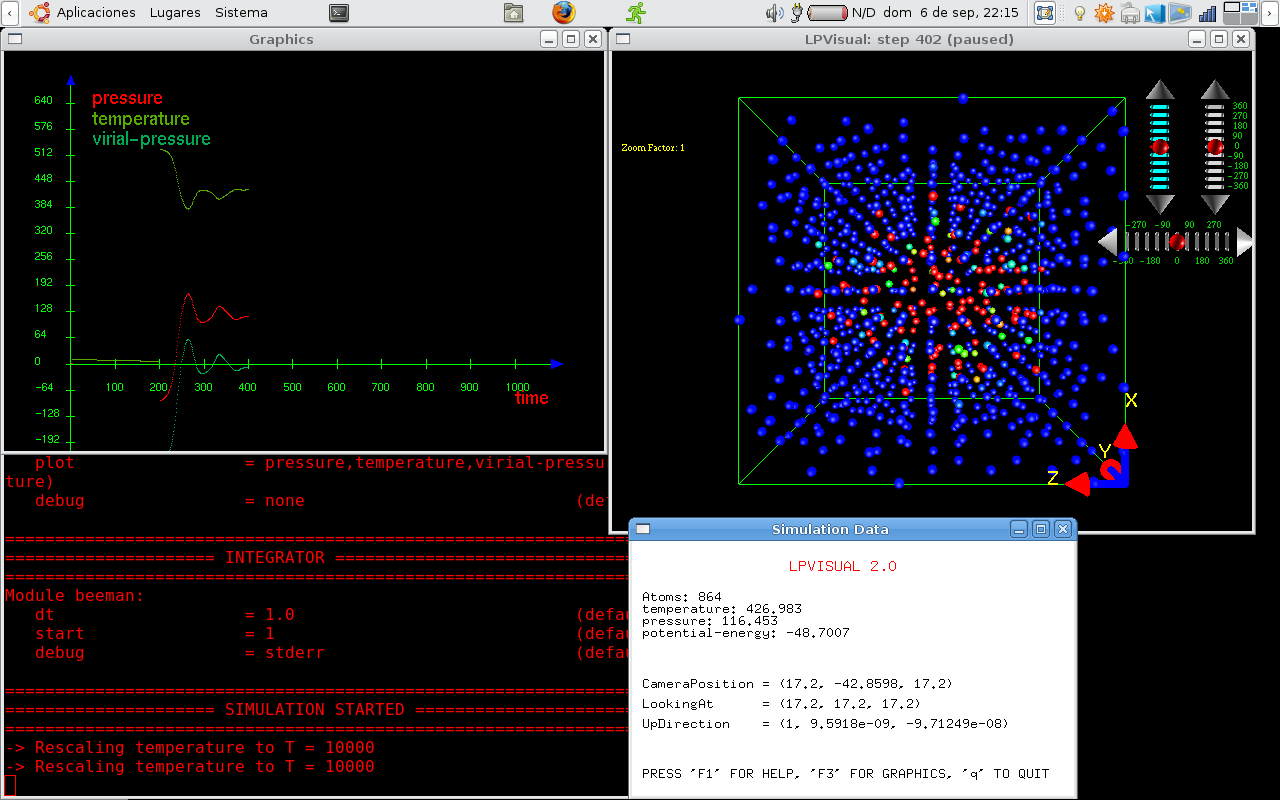
\includegraphics[width=16cm]{lpvisual1.png}
 \caption{Captura de pantalla mientras se ejecuta una simulaci\'on de din\'amica molecular con {\tt lpvisual}.}
 \label{fig:lpvisual1}
\end{figure}


\begin{figure}[h!]
 \centering
 \subfigure{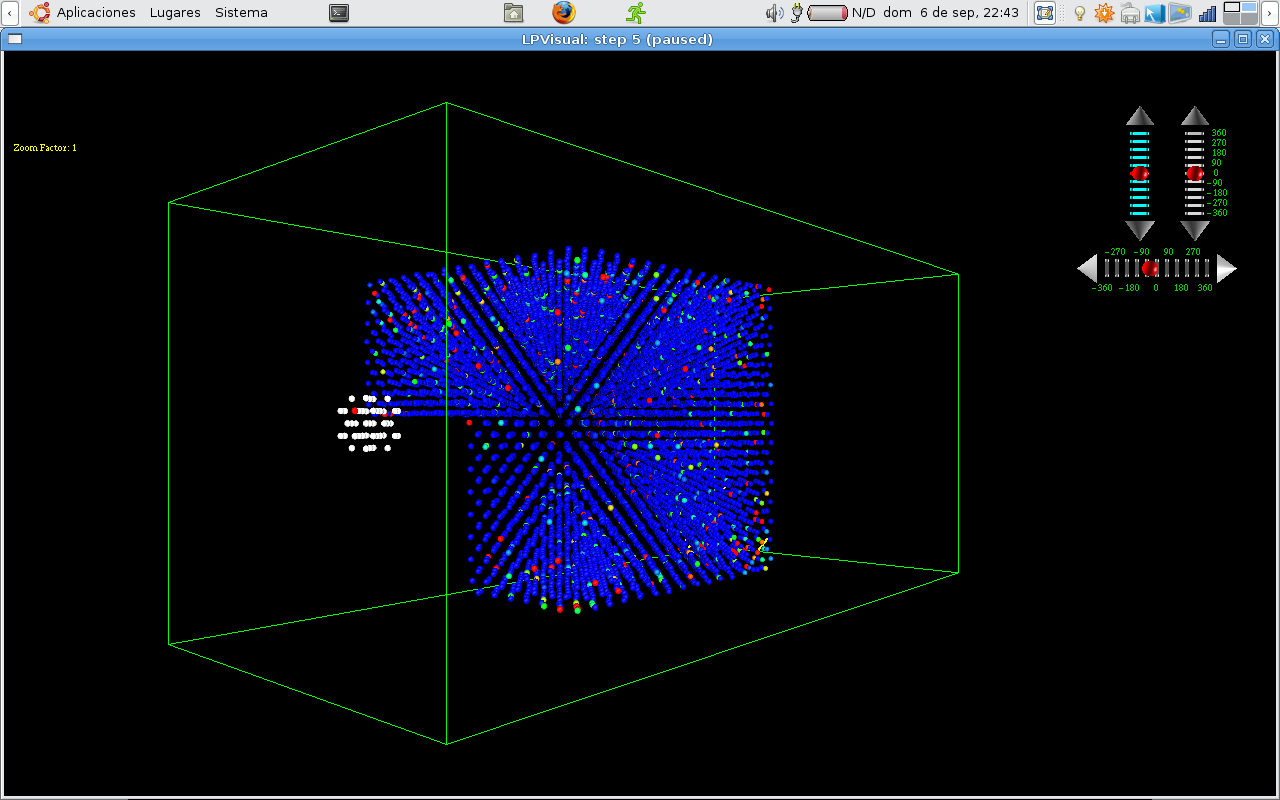
\includegraphics[width=8cm]{lpvisual2.png}}
 \subfigure{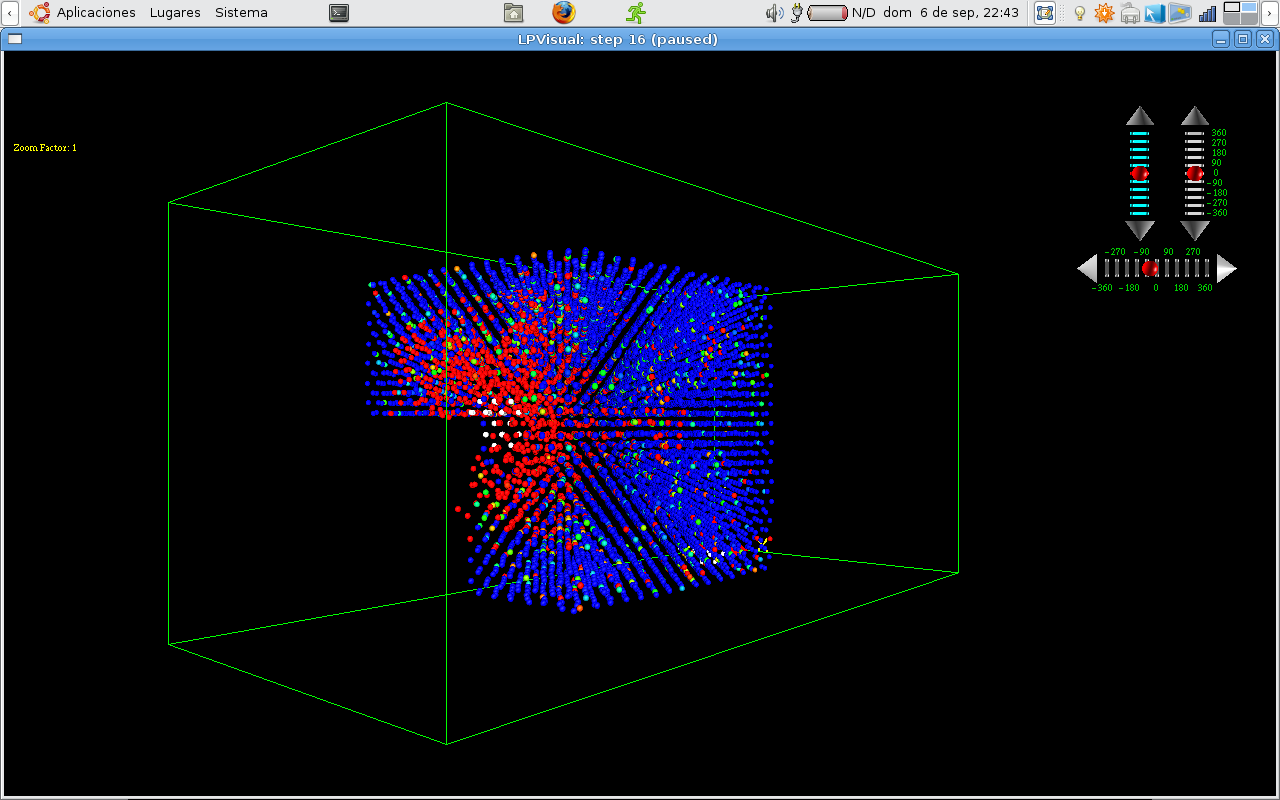
\includegraphics[width=8cm]{lpvisual3.png}}
 \subfigure{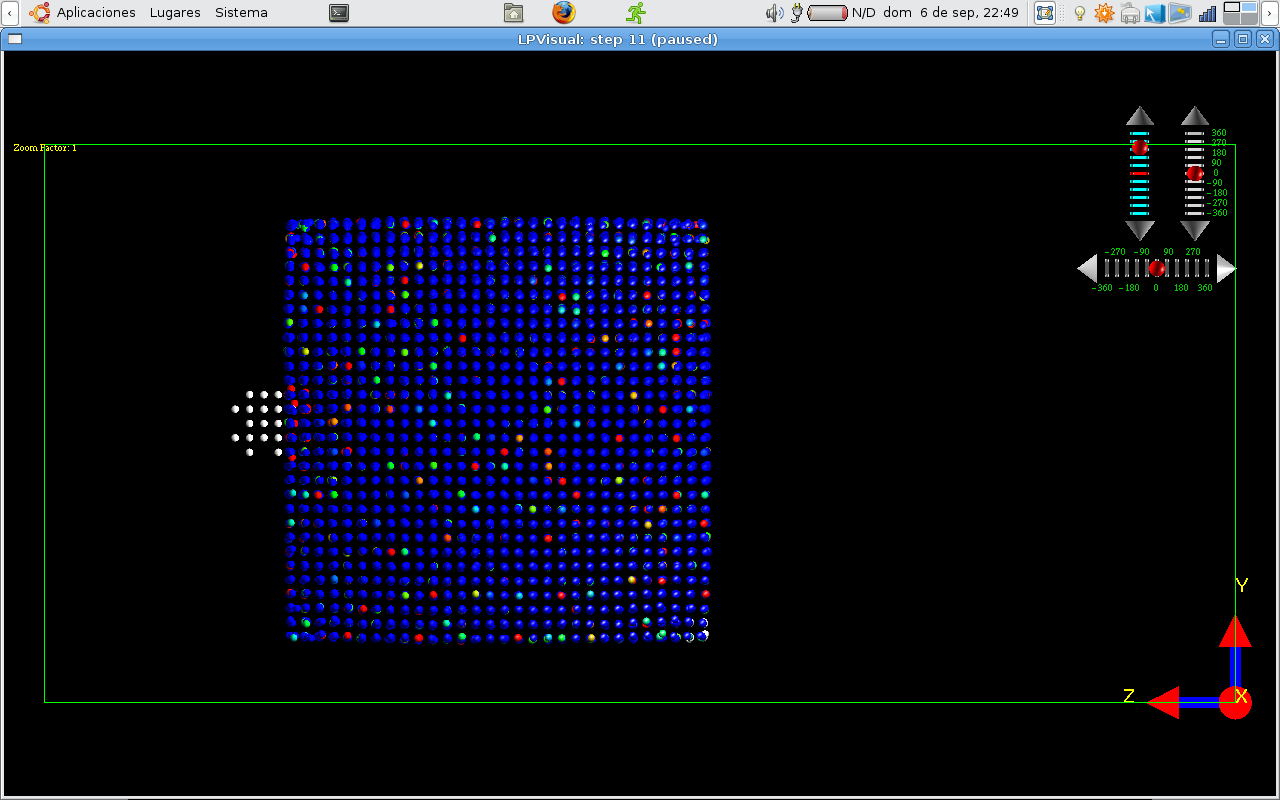
\includegraphics[width=8cm]{lpvisual4.png}}
 \subfigure{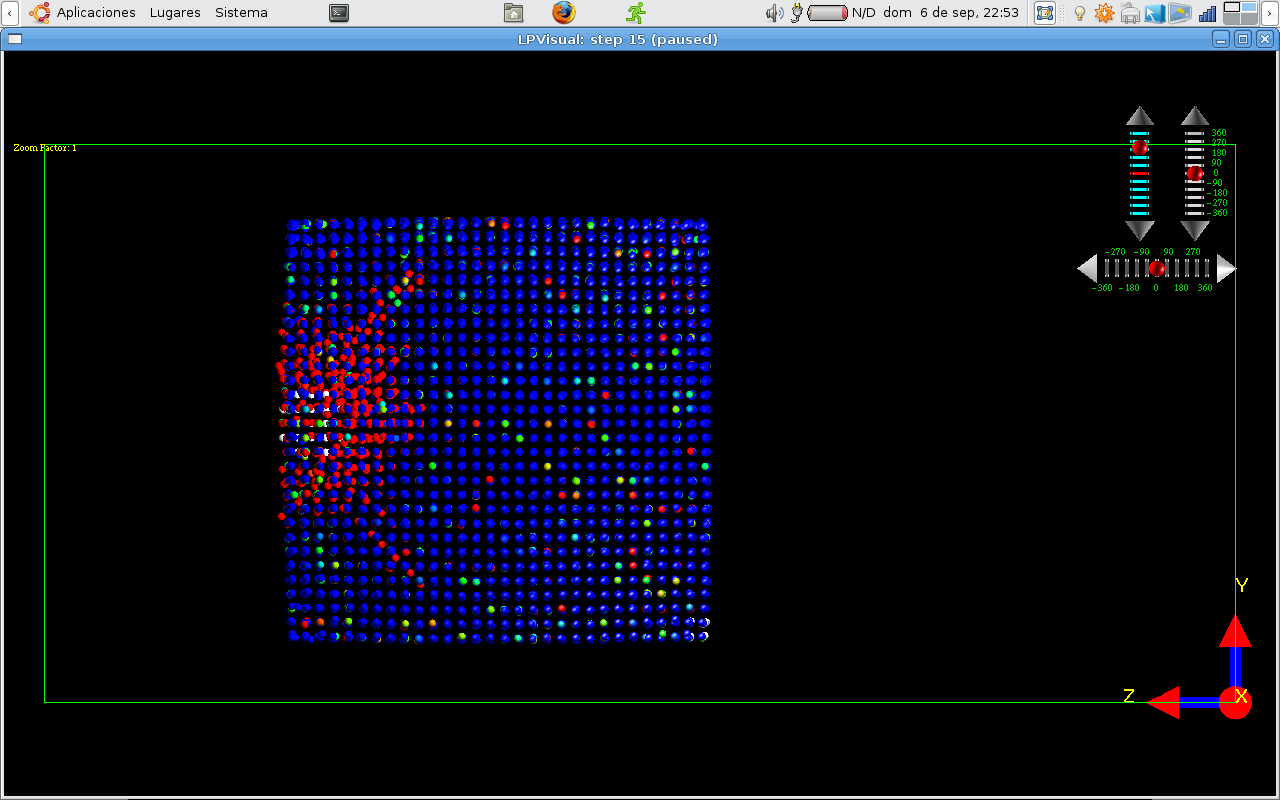
\includegraphics[width=8cm]{lpvisual5.png}}
 \label{fig:lpvisual2}
 \caption{Impacto de un proyectil sobre una celda fcc de 9000 atomos de cobre.}
\end{figure}


\newpage
\subsubsection{Opciones lpvisual}
{\bf lpvisual} ofrece varias opciones durante la visualizaci\'on que son ingresandas tanto del mouse como del teclado:\\

\begin{longtable}[fragile]{|lcp{10.5cm}|}\hline
\multicolumn{3}{|>{\columncolor[rgb]{.45,.45,.45}}c|}{Opciones del Teclado}\\\hline
\tt a&:&Esconde/muestra los ejes de coordenadas.\\
\tt c&:&Esconde/muestra los bordes de la celda de simulaci\'on.\\
\tt f&:&Pantalla completa.\\
\tt F&:&Escala la ventana a su tama\~no original.\\
\tt i&:&Esconde/muestra los controladores zoom y rotaciones.\\
\tt l&:&Cambia los bordes de la celda de simulaci\'on entre placas y espiras.\\
\tt o&:&Selecci\'on de perspectiva (ortogr\'afica / perspectiva).\\
\tt p&:&Pausa.\\
\tt q&:&Salir.\\
\tt r&:&Reset: Deshace rotaciones, movimientos, zoom (restaura la escena).\\
\tt s&:&Activa/desactiva la selecci\'on de \'atomos.\\
\tt t&:&Activa/desactiva la rotaci\'on autom\'atica.\\
\tt z&:&Comienza/detiene el acercamiento.\\
\tt Z&:&Comienza/detiene el alejamiento.\\
\tt +&:&En el modo de selecci\'on de \'atomos, va al \'atomo siguiente.\\
\tt -&:&En el modo de selecci\'on de \'atomos, va al \'atomo anterior.\\
 \tt 1->\tt 9&:&En el modo de selecci\'on de \'atomos, va al \'atomo tipeado (p. ej. ``38'').\\
{\tt CTRL}+{\tt+}&:&Aumenta el factor de zoom (el acercamiento es m\'as r\'apido).\\
{\tt CTRL}+{\tt-}&:&Disminuye el factor de zoom (el acercamiento es m\'as lento).\\
$\bs\uparrow$, $\bs\downarrow$&:&Realizan rotaciones verticales.\\
$\bs\leftarrow$, $\bs\rightarrow$&:&Realizan rotaciones horizontales.\\
{\tt SHIFT}+$\bs\uparrow$, {\tt SHIFT}+$\bs\downarrow$&:&Realizan rotaciones verticales en 5$^o$.\\
{\tt SHIFT}+$\bs\leftarrow$, {\tt SHIFT}+$\bs\rightarrow$&:&Realizan rotaciones horizontales en 5$^o$.\\
{\tt CTRL}+$\bs\uparrow$, {\tt CTRL}+$\bs\downarrow$&:&Realizan traslaciones verticales.\\
{\tt CTRL}+$\bs\leftarrow$, {\tt CTRL}+$\bs\rightarrow$&:&Realizan traslaciones horizontales.\\
{\tt F1}&:&Abre esta ventana.\\
{\tt F2}&:&Abre la ventana de datos de simulaci\'on.\\
{\tt F3}&:&Abre la ventana de gr\'aficos.\\
{\tt RePag}&:&Cambia la fuente de las letras a la pr\'oxima disponible.\\
{\tt AvPag}&:&Cambia la fuente de las letras a la anterior disponible.\\\hline
\multicolumn{3}{|>{\columncolor[rgb]{.45,.45,.45}}c|}{Opciones del Mouse}\\\hline
\multicolumn{1}{|p{4.7cm}}{Click en las flechas horizontales}&:& Rota lentamente la escena horizontalmente.\\
\multicolumn{1}{|p{4.7cm}}{Click en las flechas verticales de la esquina}&:& Rota lentamente la escena verticalmente.\\
\multicolumn{1}{|p{4.7cm}}{Click en las flechas verticales a la izquierda}&:& La camara se acerca o se aleja de la escena.\\\hline
\multicolumn{3}{|>{\columncolor[rgb]{.45,.45,.45}}c|}{Opciones de Movimiento del Mouse}\\\hline
LEFT\_MOUSE\_BUTTON&:& Al presionar esta tecla y mover el mouse simult\'aneamente, permite rotar la celda de simulaci\'on.\\
RIGHT\_MOUSE\_BUTTON&:& Al presionar esta tecla, se desplega el men\'u de la ventana activa.\\
MIDDLE\_MOUSE\_BUTTON&:&Al presionar esta tecla y mover el mouse simult\'aneamente, permite acercar (hacer $zoom$ a) la celda de simulaci\'on.\\\hline
\end{longtable}

\newpage
\subsubsection{Ejemplos}

\begin{enumerate}
\item Supongamos que tenemos un archivo \verb+configuracion.lpmd+ en donde se encuentran las posiciones at\'omicas, velocidades y colores de 9703 \'atomos de cobre en formato {\lpmd} (ver sec.~\ref{subsec:lpmdformato}). La cabecera del archivo tendr\'ia el siguiente aspecto:\\

 \begin{verbatim}
 LPMD 2.0
 HDR SYM X Y Z VX VY VZ rgb 
 9703
 70.395 0 0 0 70.395 0 0 0 150
 Cu 0.474872 0.448718 0.950733 0 0 -0.04 <1,1,1>
 Cu 0.526154 0.448718 0.950733 0 0 -0.04 <1,1,1>
 Cu 0.449231 0.474359 0.950733 0 0 -0.04 <1,1,1>
 Cu 0.474872 0.474359 0.9387 0 0 -0.04 <1,1,1>
 Cu 0.474872 0.5 0.950733 0 0 -0.04 <1,1,1>
 Cu 0.500513 0.5 0.9387 0 0 -0.04 <1,1,1>
 \end{verbatim}

Notamos que los \'atomos de cobre, en lugar de tener su color natural, aparecen con un color modificado por la \'ultima columna: \verb+<1,1,1>+, es decir, blancos. El tama\~no de esta celda es de $70.395\times70.395\times150$. Si quisieramos visualizar la configuraci\'on guardada en este archivo desde la terminal de texto, debemos llamar al manejador de visualizadores \index{lpmd-visualizer}\verb+lpmd-visualizer+ (ver sec.~\ref{sec:lpmd-visualizer}), el cual llama al visualizador \verb+lpvisual+ mediante

\control{lpmd-visualizer -i lpmd:file=configuracion.lpmd -u lpvisual -r}

El conjunto de comandos que precede a \verb+-i+ es propio del formato {\lpmd}, visto en la secci\'on~\ref{subsec:lpmdformato}. A continuaci\'on, se le pide al visualizador que utilice \verb+lpvisual+ con las opciones por defecto (nada adicional fue especificado). Por \'ultimo, el comando \verb+-r+ lee ($reads$) los vectores de celda desde dentro del archivo (el formato {\lpmd} tiene la ventaja de contener los vectores de celda, por lo que el usuario no tiene necesidad de especificarlos).

\item Supongamos que ahora deseamos visualizar una configuraci\'on de \'atomos guardada en el archivo \verb+atomos.xyz+, contenidos en una celda de $50\times20\times40$; pero esta vez queremos que la visualizaci\'on empiece con opciones distintas a las fijadas por defecto, como por ejemplo, el lugar desde donde queremos mirar la celda. En este caso, ejecutamos, por ejemplo,

\control{lpmd-visualizer -i xyz:file=atomos.xyz -u lpvisual:zenith=90,azimuth=45 -L 50,20,40}

Nuevamente, lo que precede a \verb+-i+ es propio del formato del archivo (formato \verb+xyz+ en este caso, lo que significa que debemos dar el tama\~no de celda con la opci\'on \verb+-L+). Al \verb+lpvisual+ le pasamos los \'angulos de visualizaci\'on en coordenadas polares, donde, en la notaci\'on habitual, \verb+azimuth+ es el \'angulo azimutal $\varphi$ y \verb+zenith+ es el \'angulo cenital $\theta$. En este caso, $\theta=90^o$ y $\varphi=45^o$, lo que significa que

\begin{align}
x&=\sin\theta\cos\varphi=\frac1{\sqrt2}\\
y&=\sin\theta\sin\varphi=\frac1{\sqrt2}\\
z&=\cos\theta=0
\end{align}

por lo tanto, la c\'amara se situar\'a en un vector proporcional al vector unitario $(x,y,z)=\frac{1}{\sqrt2}(1,1,0)$. La constante de proporcionalidad es el m\'odulo de la diagonal de la celda de simulaci\'on.

\item A continuaci\'on mostramos un fichero de control en donde la celda de entrada \verb+input+ (equivalente a \verb+-i+) no es un archivo, sino una celda de oro generada por el \emph{plugin} \verb+crystal3d+. En este fichero se carga \verb+lpvisual+ con todas las disponibles que \'este posee, para visualizar los primeros 10000 pasos de simulaci\'on (\verb+end=10000+):

\begin{multicols}{2}
\setlength{\columnseprule}{.5pt}
\begin{verbatim}
#######################################
# System file of Au crystal           #
# using LPMD                          #
#######################################

cell cubic 32.08
input crystal3d \
       type=fcc symbol=Au nx=8 ny=8 nz=8
output module=lpmd \
	      file=au.lpmd each=15 level=1
periodic true true true
steps 750000


monitor properties=step,kinetic-energy,\
        potential-energy,virial-pressure,\
	total-energy,temperature \
	output=au.out start=0 end=750000 each=1

######################################
########## Integrator ################
######################################

use velocityverlet
 dt 1.0
enduse

######################################
############ CellManager #############
######################################

use linkedcell
 mode auto
 cutoff 7.5
enduse

#######################################
########## Potential ##################
#######################################

# Parameters for gold
use suttonchen as sc
 e 0.013
 n 10
 a 4.08
 m 8
 c 34.408
 cutoff 7.1
enduse



######################################
######### Tempscaling ################
######################################

#Aplicar un escalamiento de t de 300K
prepare temperature t=300.0

use tempscaling as tmpsc
 from 300
 to 300
enduse


######################################
######### CellScaling ################
######################################

#Estirar la celda
use cellscaling as cs
 percent 1
enduse

######################################
######### Visualization ##############
######################################

#Visualizar la simulacion
use lpvisual
 width  640
 height 480
 radius 0.5
 quality 3
 azimuth 0.0
 zenith -90.0
 background white
 autorotate true
 perspective false
 properties potential-energy,kinetic-energy
 plot total-energy,temperature
enduse

#--------------------------------------#
#           use plugins                #
#--------------------------------------#
cellmanager linkedcell
integrator velocityverlet
potential sc Au Au
apply cs start=70000 end=700000 each=70000
apply tmpsc start=0 end=20000 each=50
visualize lpvisual start=0 end=10000 each=1


\end{verbatim}
\end{multicols}

- Esto visualiza la simulaci\'on cada 50 pasos (each) durante los primeros 10000 pasos (\verb+end+) de simulacion, comenzando desde el paso inicial (\verb+start+).\\

- Los par\'ametros \verb+width+ y \verb+heigh+ dan el ancho de la ventana deseados, mientras que \verb+radius+ y \verb+quality+ dan el radio de los atomos y su calidad (que tan parecidos a una esfera ser\'an), respectivamente.\\

- Con \verb+azimuth+ ($\varphi$) y \verb+zenith+ ($\theta$) podemos dar las coordenadas esf\'ericas angulares que determinan el vector posicion inicial de la camara.\\

- Con \verb+backgroun+, elegimos el fondo de la pantalla blanco (\verb+white+). Fondos disponibles: white, gray, orange, black (default).\\

- Con \verb+autorotate+, iniciamos la simulacion en rotaci\'on automatica.\\

- \verb+perspective+ inicia una visualizaci\'on ortorombica (\verb+perspective=false+).\\

- Finalmente, \verb+properties+ son las propiedades cuyo valor numerico sera monitoreado en una ventana secundaria del visualizador, mientras que \verb+plot+ ser\'an las propiedades que se graficar\'an en otra ventana independiente mientras transcurre la simulaci\'on.                         

\end{enumerate}


